\chapter{Method}

\section{Synthetic data - Collect data from CARLA}

\begin{comment}

Premise: Have no data to train a NeRF on
Question: How can we collect synthetic data from CARLA?

\begin{itemize}
    \item How can you spawn an agent, etc?
    \item How does all the basic CARLA-things work? 
    \item How to mount cameras, which sensors, location and rotation (transform).
\end{itemize}
\end{comment}

% Code: generic_nerf_capture.py
\subsubsection{Connecting the CARLA API to a CARLA simulator}
I might add something here about how the data flows in the CARLA setup.



\subsubsection{Creating a CARLA Actor}
In order to capture data we need a programmable vehicle that we control, usually referred to as the \textit{ego} vehicle. An ego vehicle, \texttt{carla.Vehicle} is a special instance of the most basic CARLA instance, the \texttt{carla.Actor}. It can be spawned by defining a spawn point, a choice of vehicle, and whether the vehicle should run on autopilot or not. An arbitrary amount of autopilot vehicles can be spawned in order to simulate a complex traffic environment, but we want to capture synthetic data with the least amount of transient objects so we only spawn the ego vehicle.


\subsubsection{Setting up the environment with the traffic manager}

In order to define the environment in which the spawned ego vehicle will operate, we leverage the \texttt{carla.TrafficManager} available on the \texttt{carla.Client} that's used to connect to the simulator. The traffic manager enables us to define some important aspects of the environment:

\begin{itemize}
    \item \textbf{Choose the ego vehicle's route:} The traffic manager allows us to set the route instructions for a certain actor. We can define arbitrary routes by creating an array of route instructions, e.g. \texttt{['Left', 'Left', 'Right', 'Straight', 'Right']}.
    \item \textbf{Ignore the traffic lights:} Since the only moving vehicle in the environment is the ego vehicle, we don't have to abide by the rules of traffic. In order to speed up the data capture we choose to ignore the traffic lights.
    \item \textbf{Set the vehicle speed:} The traffic manager allows us to set a vehicle's speed to a percentage of the default speed of 30 km/h. When set to $100$ we follow the default speed of 30 km/h, when set to $50$ the speed will be 15 km/h, etc.
\end{itemize}


\subsubsection{Run configuration}

In order to test multiple configurations of environment and vehicle setup and the corresponding results, I created an \texttt{ExperimentSetting}-class. It enables the following configurations:

\begin{itemize}
    \item \textbf{Defining a camera rig:} Mounts a list of RGB-cameras with configurable camera settings, location and rotation to the ego vehicle. We're optionally able to parse a rig file exported from the NAPLab car into a camera rig for the ego vehicle.
    \item \textbf{Camera frame rate}: Sets the rate of image capture.
    \item \textbf{Stop-criteria:} Specifies the ego vehicle's stop condition either by a stop distance or a number of completed turns.
    \item \textbf{Camera noise:} Enables the simulation of noisy GPS/GNSS sensor readings by adding Gaussian noise to the location/rotation output from the mounted cameras.
    \item \textbf{Spawn transform:} Enables specifying the spawn-location/-rotation of the ego vehicle.
    \item \textbf{Vehicle speed.} Sets the vehicle speed for the ego vehicle.
    \item \textbf{Path:} Sets the route instructions for the ego vehicle.
\end{itemize}


\subsubsection{TransformFile}

Create an instance of \texttt{TransformFile} used to store the images and corresponding camera poses from the camera rig mounted to the car. We’ll explore the details behind the format and data conventions in \autoref{sec:carla-to-nerfstudio}.

\subsubsection{CARLA Run-loop}
The CARLA Run-loop includes the following steps:

\begin{itemize}
    \item While the car hasn’t met a stop-criteria, e.g. that it has driven the set amount of distance/turns, keep driving and collecting data.
    \begin{itemize}
        \item \textbf{Get the image from all the cameras mounted to the car:} Every carla sensor has a \texttt{listen} method which is called every time a sensor retrieves data. \textit{Carlo} (\textbf{add citation}) has abstracted the pipeline for retrieving image data from a respective camera, which would otherwise require handling the listen-callback, reading of the \texttt{carla.Image} data and transform from raw data (bytes) to \texttt{np.ndarrays}. With the Carlo-abstraction, I only need to create a list of cameras, get the \texttt{np.ndarray} containing the image-data, stack the camera output and display the respective image with a tool like \texttt{cv2}.
    \end{itemize}
    \item Store the image-/camera pose data if it’s the correct tick
\end{itemize}


The following algorithm outlines the steps for capturing synthetic data using the CARLA simulator. The code is written in Python and utilizes the CARLA library.

\begin{comment}
    
\begin{algorithmic}[1]
\Function{run\_carla\_session}{experiment\_settings}
    \State \textbf{create a directory} for the experiment and save experiment settings to a file
    \State \textbf{create a SLURM script} for the experiment
    \State \textbf{spawn an ego vehicle} and set up the traffic manager
    \State \textbf{create cameras} based on the specified camera rigs and rig file
    \State \textbf{create a TransformFile} to store the image and camera pose data
    \While{\textbf{stop criteria has not been met}}
        \State \textbf{tick the CARLA world}
        \State \textbf{get images} from all mounted cameras and stack them horizontally
        \State \textbf{show the image}
        \State \textbf{store the image and camera pose data} every n-th tick
        \State \textbf{update the distance traveled} using euclidean distance
    \EndWhile
    \State \textbf{export the TransformFile} and destroy the actors
\EndFunction
\end{algorithmic}

\end{comment}











\section{From CARLA to Nerfstudio} \label{sec:carla-to-nerfstudio}
\begin{comment}
Premise: Have collected data from CARLA.
Question: How do I get it from CARLA to Nerfstudio in a usable format?

\begin{itemize}
    \item Use the CARLA-simulator to find out which camera and vehicle settings work the best for capturing data for NeRFs.
    \item In order to do that I need to collect data from CARLA and convert it into a format that's usable by Nerfstudio.
\end{itemize}
\end{comment}

We now have a pipeline that enables the creation of a controllable environment for a vehicle with an arbitrary setup of sensors. How do we export the collected sensor data in a format that's readable by Nerfstudio?

In order to train a NeRF we need images and corresponding camera poses. As discussed in \autoref{sec:nerf}, the camera poses are $4x4$ homogeneous transformation matrices, containing both the translation and rotation in reference to a coordinate system. Nerfstudio expects a file structure as shown in \autoref{fig:nerfstudio-file-structure}. In order to handle the data parsing from CARLA to Nerfstudio we create a helper-class \texttt{TransformsFile} which have methods for saving images as PNG-files, calculating the camera's intrinsic parameters, transforming the extrinsic parameters, and appending parsed frames to the \texttt{transforms.json}-file.

\begin{figure}[ht]
\centering
\begin{forest}
for tree={
      parent anchor=south west,
      child anchor=west,
      anchor=mid west,
      inner ysep=1pt,
      grow'=0,
      align=left,
      edge path={
        \noexpand\path [draw, \forestoption{edge}] (!u.parent anchor) ++(1em,0) |- (.child anchor)\forestoption{edge label};
      },
      font=\sffamily,
      if n children=0{}{
        delay={
          prepend={[,phantom, calign with current]}
        }
      },
      fit=band,
      before computing xy={
        l=2em
      }
    }
[ your\_nerf\_data/
  [ images/
    [ 0001.png ]
    [ 0002.png ]
    [ 0003.png ]
    [ \ldots{} ]
  ]
  [ transforms.json ]
]
\end{forest}
\caption{File structure expected by Nerfstudio}
\label{fig:nerfstudio-file-structure}
\end{figure}

CARLA gives access to basic camera attributes that we can use to approximate the intrinsic parameters. Given the image's width $w$ and height $h$, in accordance to the camera's field of view $fov$, we can calculate the focal length $f$ and subsequently the $x$- and $y$-component of the focal length $f_x$ and $f_y$ as follows:

\begin{align*}
f &= \tan\left(\frac{\text{fov}}{2}\right) &
f_x &= \frac{0.5 \times w}{f} &
f_y &= \frac{0.5 \times h}{f}
\end{align*}

The camera's principal points $c_x$ and $c_y$ are assumed to be the center of the image plane, and obtained with:

\begin{align*}
c_x &= \frac{w}{2} &
c_y &= \frac{h}{2}
\end{align*}

The calculated intrinsic values will then be added to a \texttt{transforms.json}-file that contains the camera's intrinsics and a list of frames where each frame has a reference to an image and that image's camera pose. An example \texttt{transforms.json}-file can be seen in \autoref{code:transform-examples}.

\begin{figure}[ht]
\centering
\begin{lstlisting}[language=json,linewidth=0.9\linewidth]
{
    "camera_model": "OPENCV",
    "fl_x": 200.0,
    "fl_y": 150.0,
    "cx": 200.0,
    "cy": 150.0,
    "w": 400,
    "h": 300,
    "k1": 0,
    "k2": 0,
    "p1": 0,
    "p2": 0,
    "frames": [...]
}
\end{lstlisting}
\caption{Example of a \texttt{transforms.json}-file with the intrinsic parameters and a collapsed list of frames containing the extrinsic parameters of the camera.}
\label{code:transform-examples}
\end{figure}


CARLA is built with Unreal Engine and subsequently uses its coordinate convention, with some noticeable differences which we'll get back into later. The Unreal Engine coordinate convention is a left-handed system with the up vector being +Z. Nerfstudio uses the OpenGL/Blender coordinate convention for cameras, which is a right-handed system, and its world space is oriented such that the up vector is +Z. The disparity in coordinate conventions between CARLA and Nerfstudio would make the NeRF-renderings non-interpretable, if we trained a NeRF directly on the transformation matrices exported from CARLA. In order to transform the transformation matrices that contain both rotation and translation we apply \texttt{TransformFile}'s \texttt{carla\_to\_nerf}-transformation as described in \textbf{INSERT FIGURE/EQUATION HERE}, before appending the frame to the \texttt{transform.json}-file. The \texttt{carla\_to\_nerf} function takes a \texttt{carla.Transform} object as input and returns a 4x4 matrix in OpenGL/Blender-format. The function first extracts the location and rotation components of the input transform. The location component is then converted from the Unreal Engine coordinate system to the OpenGL/Blender coordinate system used by Nerfstudio. This conversion involves swapping the X and Y coordinates of the location and negating the Z coordinate. The rotation component is also converted to the OpenGL/Blender coordinate system by swapping the pitch and roll angles and adding 90 degrees to each angle. Finally, the transformed location and rotation components are combined into a new \texttt{carla.Transform} object, which is used to generate the 4x4 matrix that is returned by the function. An example of the transformed CARLA-matrix can be seen in \autoref{code:frame-example}.

\begin{figure}[ht]
    \centering
    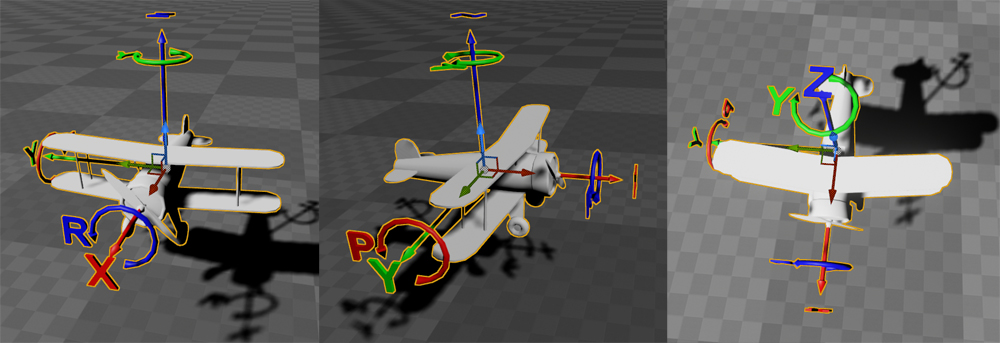
\includegraphics[width=1.0\textwidth]{figures/carla-coordinates-system.jpeg}
    \caption[Overview of CARLA's coordinates system]{CARLA uses the Unreal Engine's coordinates system, which is a Z-up left-handed system \cite{carla-coordinates-system}.}
    \label{fig:carla-coordinates-system}
\end{figure}
\begin{figure}[ht]
\centering
\begin{lstlisting}[language=json,linewidth=0.9\linewidth]
{
  "file_path": "images/0001.png",
  "transform_matrix": [
    [-0.0914, -0.9461, -0.3106, -1.6014],
    [ 0.9953, -0.0967,  0.0014, 106.6598],
    [-0.0314, -0.3090,  0.9506, -2.9952],
    [ 0.0000,  0.0000,  0.0000,  1.0000]
  ]
}
\end{lstlisting}
\caption{Example of a frame from a \textit{transforms.json}-file, containing a reference to a image and that image's camera pose as a transformation matrix.}
\label{code:frame-example}
\end{figure}



\begin{comment}
% TODO: In order to use these matrices I need to make sure they're correct

$$
\begin{bmatrix}
x_{blender} \\ y_{blender} \\ z_{blender} \\ 1
\end{bmatrix}
=
\begin{bmatrix}
0 & -1 & 0 & 0 \\
1 & 0 & 0 & 0 \\
0 & 0 & -1 & 0 \\
0 & 0 & 0 & 1
\end{bmatrix}
\begin{bmatrix}
x_{unreal} \\ y_{unreal} \\ z_{unreal} \\ 1
\end{bmatrix}
$$




where $(x_{blender}, y_{blender}, z_{blender})$ are the coordinates of the camera location in the Blender coordinate system, $(x_{unreal}, y_{unreal}, z_{unreal})$ are the coordinates of the camera location in the Unreal Engine coordinate system, $(\phi_{blender}, \theta_{blender}, \psi_{blender})$ are the Euler angles of the camera rotation in the Blender coordinate system, and $(\phi_{unreal}, \theta_{unreal}, \psi_{unreal})$ are the Euler angles of the camera rotation in the Unreal Engine coordinate system.




Sure! Here's the transformation from a `carla.Transform` to a 4x4 matrix in LaTeX matrix form:

Let $\mathbf{p}_{\text{CARLA}} = (x_{\text{CARLA}}, y_{\text{CARLA}}, z_{\text{CARLA}})$ be the location vector in CARLA coordinates, and let $\mathbf{R}_{\text{CARLA}}$ be the rotation quaternion in CARLA coordinates. We can convert $\mathbf{p}_{\text{CARLA}}$ and $\mathbf{R}_{\text{CARLA}}$ to a 4x4 transformation matrix $\mathbf{T}_{\text{NerfStudio}}$ as follows:

1. Translate $\mathbf{p}_{\text{CARLA}}$ by $(0, 0, z_{\text{CARLA}})$ to align the Z-axes of the two coordinate systems. This can be represented by the following translation matrix:

$$
\mathbf{T}_1 =
\begin{bmatrix}
1 & 0 & 0 & 0 \\
0 & 1 & 0 & 0 \\
0 & 0 & 1 & z_{\text{CARLA}} \\
0 & 0 & 0 & 1
\end{bmatrix}
$$

2. Rotate $\mathbf{R}_{\text{CARLA}}$ by $90^\circ$ around the X-axis to convert from a Z-up left-handed system to a Y-up right-handed system, and swap the pitch and roll components to account for the different order of declaration in the Unreal Engine and Blender coordinate systems. This can be represented by the following rotation matrix:

$$
\mathbf{T}_2 =
\begin{bmatrix}
1 & 0 & 0 & 0 \\
0 & 0 & 1 & 0 \\
0 & -1 & 0 & 0 \\
0 & 0 & 0 & 1
\end{bmatrix}
\begin{bmatrix}
1 & 0 & 0 & 0 \\
0 & 0 & 1 & 0 \\
0 & -1 & 0 & 0 \\
0 & 0 & 0 & 1
\end{bmatrix}
=
\begin{bmatrix}
1 & 0 & 0 & 0 \\
0 & 0 & -1 & 0 \\
0 & 1 & 0 & 0 \\
0 & 0 & 0 & 1
\end{bmatrix}
$$

3. Swap the Y and Z coordinates of $\mathbf{p}_{\text{CARLA}}$ to account for the different orientation of the Y and Z axes in the two coordinate systems. This can be represented by the following matrix:

$$
\mathbf{T}_3 =
\begin{bmatrix}
1 & 0 & 0 & 0 \\
0 & 0 & 1 & 0 \\
0 & 1 & 0 & 0 \\
0 & 0 & 0 & 1
\end{bmatrix}
$$

4. Rotate $\mathbf{R}_{\text{CARLA}}$ by $-90^\circ$ around the Z-axis to convert from a Y-up right-handed system to a Z-up right-handed system. This can be represented by the following rotation matrix:

$$
\mathbf{T}_4 =
\begin{bmatrix}
0 & 1 & 0 & 0 \\
- 1 & 0 & 0 & 0 \\
0 & 0 & 1 & 0 \\
0 & 0 & 0 & 1
\end{bmatrix}
$$

5. The resulting matrix $\mathbf{T}_{\text{NerfStudio}}$ is obtained by multiplying these matrices together in the following order:

$$
\mathbf{T}_{\text {NerfStudio}} = \mathbf{T}_4 \mathbf{T}_3 \mathbf{T}_2 \mathbf{T}_1
$$

This gives us the 4x4 transformation matrix that can be used in NerfStudio.





Let $\mathbf{R}_{\text{CARLA}}$ be the rotation matrix in CARLA coordinates, and let $\mathbf{R}_{\text{NerfStudio}}$ be the corresponding rotation matrix in NerfStudio coordinates. We can transform $\mathbf{R}_{\text{CARLA}}$ into $\mathbf{R}_{\text{NerfStudio}}$ using a series of elementary rotations.

First, we rotate $\mathbf{R}_{\text{CARLA}}$ by $90^\circ$ around the X-axis to convert from a Z-up left-handed system to a Y-up right-handed system. This rotation can be represented by the following matrix:

$$
\mathbf{R}_1 =
\begin{bmatrix}
1 & 0 & 0 \\
0 & 0 & 1 \\
0 & -1 & 0
\end{bmatrix}
$$

Next, we swap the Y and Z coordinates of $\mathbf{R}_{\text{CARLA}}$ to account for the different orientation of the Y and Z axes in the two coordinate systems. This can be accomplished by multiplying $\mathbf{R}_{\text{CARLA}}$ on the left by the following matrix:

$$
\mathbf{R}_2 =
\begin{bmatrix}
1 & 0 & 0 \\
0 & 0 & 1 \\
0 & 1 & 0
\end{bmatrix}
$$

Finally, we rotate $\mathbf{R}_{\text{CARLA}}$ by $-90^\circ$ around the Z-axis to convert from a Y-up right-handed system to a Z-up right-handed system. This rotation can be represented by the following matrix:

$$
\mathbf{R}_3 =
\begin{bmatrix}
0 & 1 & 0 \\
- 1 & 0 & 0 \\
0 & 0 & 1
\end{bmatrix}
$$

To obtain $\mathbf{R}_{\text{NerfStudio}}$, we can multiply these matrices together in the following order:

$$
\mathbf{R}_{\text{NerfStudio}} = \mathbf{R}_3 \mathbf{R}_2 \mathbf{R}_1 \mathbf{R}_{\text{CARLA}}
$$

This gives us the rotation matrix that we can use to construct a NerfStudio transform.
\end{comment}















\section{Nerfstudio pipeline with CARLA-data} \label{sec:nerfstudio-pipeline}
\begin{comment}
Premise: Have data in a Nerfstudio format, collected from CARLA.
Question: How can I train a NeRF that represent the same scene?

\begin{itemize}
    \item Explain the Nerfstudio API and the created pipeline. Train, eval, render
    \item Go into detail on e.g. the train/eval-split, training parameters, etc. Add additional info to the appendix.
\end{itemize}
\end{comment}

We now have the synthetic data captured from CARLA in a format that we can use to train NeRFs in Nerfstudio on. How do I use this data and the Nerfstudio API to create a pipeline that automates processing, training, evaluating and rendering the different experiments?

I've created a pipeline that leverage the Nerfstudio API to process, train, evaluate and render the NeRFs. The pipeline accepts parameters including:

\begin{itemize}
    \item \textbf{Input/output directory:} Defines where the data is located and where the output from the pipeline should be stored?
    \item \textbf{Model:} Defines which model to use for training the NeRF
    \item \textbf{Settings for camera optimizer:} Defines if the NeRF should also treat the camera poses as learnable parameters and optimize the camera poses.
    \item \textbf{Settings for side-by-side rendering:} Defines, among other things, which input-camera should be used as ground truth when rendering side-by-side.
\end{itemize}

\subsubsection{Process}

In most scenarios when working with real data, e.g. images of an object captured with a handheld camera, we don't have accurate camera poses. In those scenarios we have to pre-process the data in order to approximate camera poses for the captured images. It can be accomplished by leveraging SfM-algorithms as explained in \autoref{sec:sfm}. In the scenario where we're dealing with synthetic data captured from CARLA, the poses are as accurate as they can be as they've been calculated in a deterministic environment. Due to this, and the fact that we've already parsed the data into a Nerfstudio data format as shown in \autoref{fig:nerfstudio-file-structure} and \autoref{code:transform-examples}, we don't have to do any preprocessing.

\subsubsection{Train}

The experiments in this thesis focus on the faster NeRF models implemented in Nerfstudio, namely Nerfacto (\autoref{sec:nerfacto}) and Instant NGP (\autoref{sec:instant-ngp}). Although the models are different, most of the shared model configurations are the same as can be seen in the model parameters included in \autoref{sec:nerfstudio-train-parameters}. During training, the parameters in the model are trained to represent the 3D scene. For the Nerfacto-model, this entails backpropagating the error and updating both the NeRF MLP and the proposal MLP.

The Nerfacto- and Instant NGP-model leverage 3 different losses to guide the training; \textit{RGB loss}, \textit{interlevel loss} and \textit{distortion loss}. \textit{RGB loss} is the standard NeRF-loss explained in \autoref{eq:nerf-loss}. Interlevel- and distortion-loss are both from the Mip-NeRF 360 implementation explained in \autoref{sec:mipnerf360}. The interlevel loss encourages the model to generate consistent predictions across different levels of the multi-scale hierarchy, while the distortion loss encourages the model to generate smooth and continuous predictions.

The training leverages the ADAM optimizer for all networks within the model. The optimizer for the proposal networks and Nerfacto fields both use a learning rate of $1 \times 10^{-2}$, with no weight decay and $\epsilon=10^{-8}$, while the camera optimizer use a learning rate of $6 \times 10^{-4}$, weight decay of $1 \times 10^{-2}$, and $\epsilon=10^{-8}$. All scenes were trained for 15,000 iterations, which is sufficient for achieving convergence. Training time for each scene is approximately 15-20 minutes when using an NVIDIA A100 GPU.

% TODO: Rewrite and reorganize. Write about how a batch of pixels are created for each training iteration
During the training of a NeRF, a batch of pixels is created for each training iteration. By default, this batch consists of 4096 pixels. To obtain these pixels, the training algorithm randomly samples them from all of the training images that are stored in RAM. However, this approach can be memory-intensive, especially when dealing with large datasets. To address this issue, the NeRF pipeline provides an option to set the parameter \texttt{–-pipeline.datamanager.train-num-images-to-sample-from}, which allows the user to sample pixels from a smaller subset of images. When using a smaller subset of images, the training algorithm will keep sampling from this subset unless the parameter \texttt{--num-times-to-repeat-images} is also set. This parameter specifies the number of training iterations after which the training algorithm should grab a new set of images to sample from. For instance, if \texttt{--num-times-to-repeat-images} is set to 1, the training algorithm will grab a new set of images to sample from every iteration. However, this approach can be computationally expensive and slow down the training process.

\subsubsection{Evaluate}

To evaluate the quality of the NeRF models, we employ the metrics discussed in \autoref{sec:evaluating-nerfs}, including PSNR, SSIM, and LPIPS. The Nerfstudio API provides a script to load a checkpoint and compute these metrics, providing a quantitative assessment of the trained NeRF. To facilitate the comparison of NeRF models across multiple experiments, a script was developed to load the evaluation outputs, compare the resulting metrics, and produce a formatted LaTeX table that highlights the best and worst-performing models. While these metrics offer valuable insights into the quality of the model, there is also significant value in the qualitative output. Therefore, we also render all trained NeRF models to visually compare the results across different methods, configurations, and datasets.

\begin{figure}[h]
    \centering
    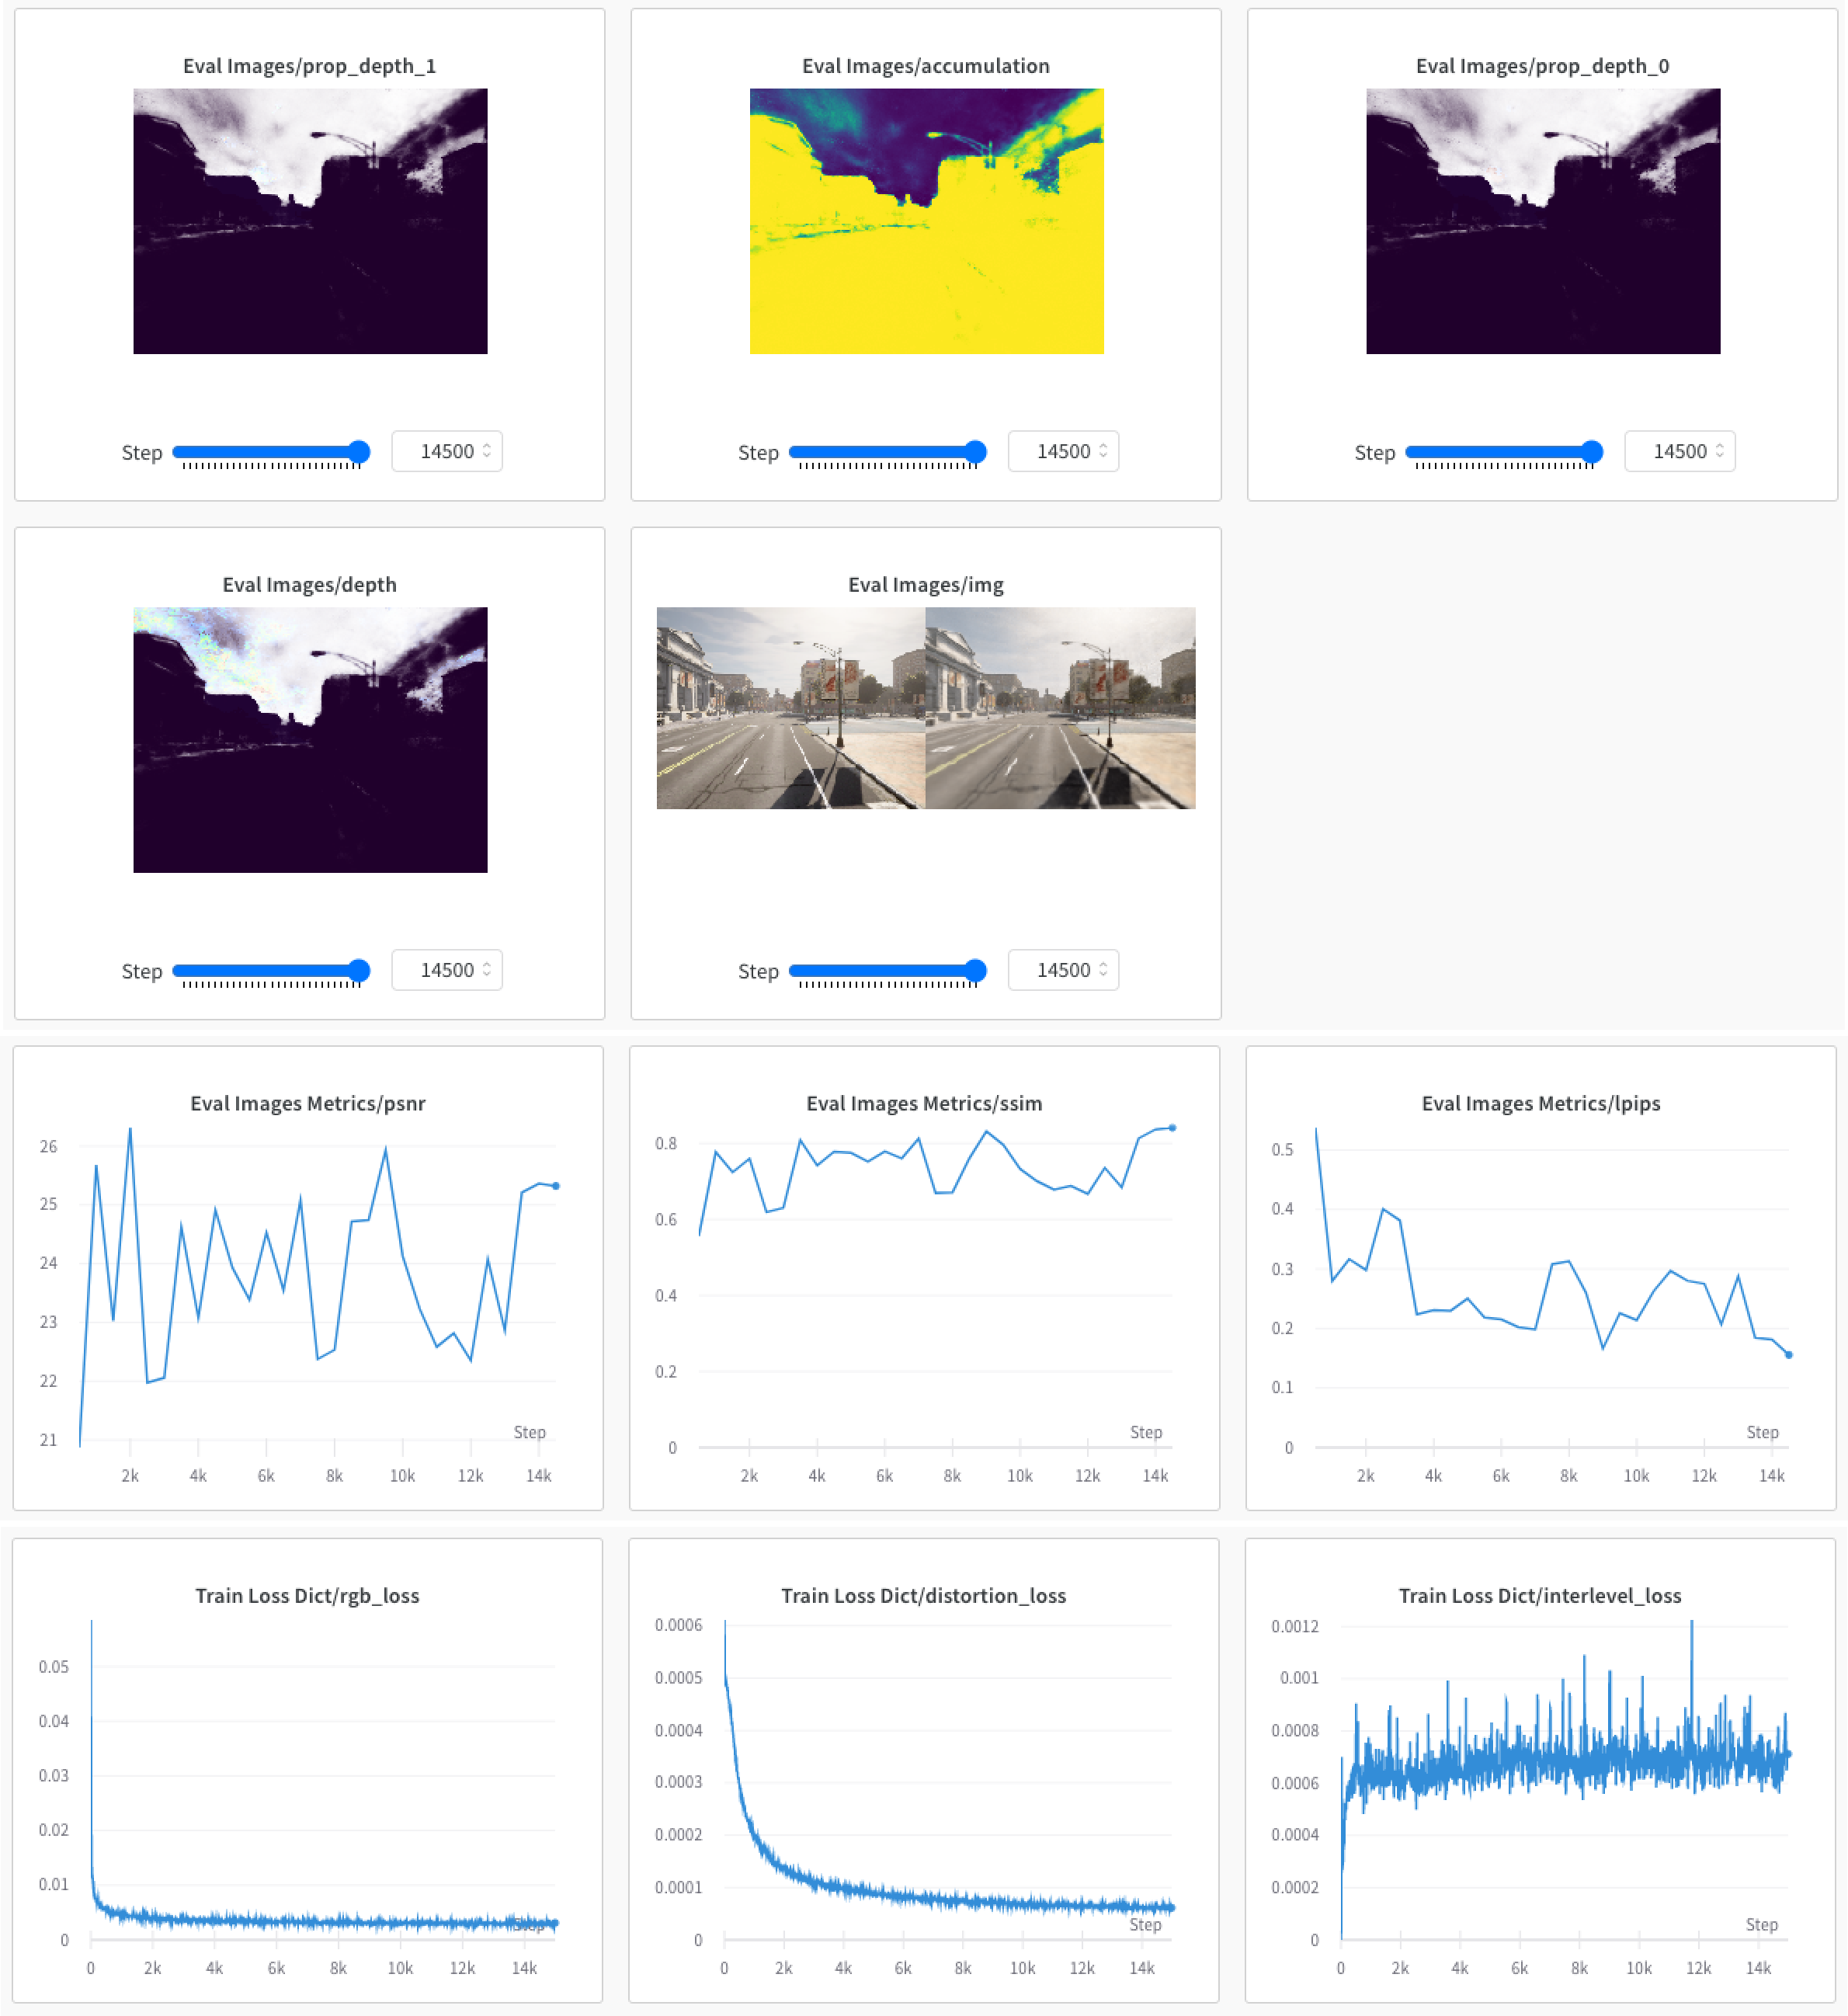
\includegraphics[width=1.0\textwidth]{figures/wandb-eval-data.png}
    \caption{Selection of evaluation data from Weights \& Biases \cite{wandb} for a NeRF training on a segment of synthetic data from CARLA.}
    \label{fig:wandb-eval-data}
\end{figure}

\subsubsection{Render} % FIX: the reasoning for why side-by-side was created

The Nerfstudio API provides a script for rendering trained NeRF models given a sequence of camera positions, each with a corresponding field of view and aspect ratio, as shown in the camera path example in \autoref{code:camera-path-example}. The Nerfstudio viewer, depicted in \autoref{fig:nerfstudio-viewer-overview}, enables the creation and editing of camera paths, which can be exported and used for rendering. However, comparing experiments across different models and datasets with custom camera paths that will be slightly different for run/scene can be time-consuming and challenging. To address this issue, a script was developed to extract the ground truth camera path and use it in conjunction with the input images and trained NeRF model to create a side-by-side rendering. This approach has proven to be a useful means of qualitatively evaluating the performance of the NeRF models.

% TODO: Write about the side-by-side script

\begin{figure}[H]
    \centering
    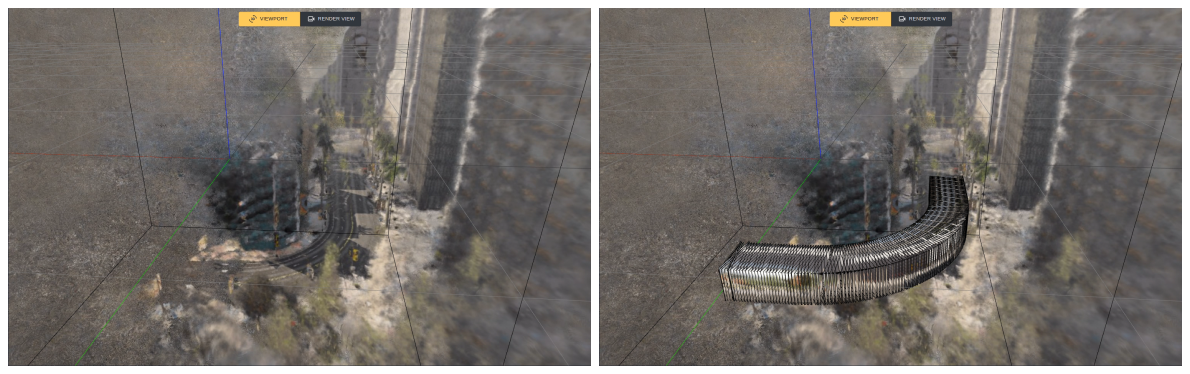
\includegraphics[width=1.0\textwidth]{figures/nerfstudio-viewer-overview.png}
    \caption{An overview of the Nerfstudio viewer. The scene seen on the left has been trained on the set of images and camera poses revealed in the image to the right.}
    \label{fig:nerfstudio-viewer-overview}
\end{figure}
\begin{figure}[ht]
\centering
\begin{lstlisting}[language=json,linewidth=0.9\linewidth]
{
  "camera_type": "perspective",
  "render_height": 1080,
  "render_width": 1920,
  "fps": 24,
  "seconds": 10,
  "smoothness_value": 0.4624,
  "is_cycle": true,
  "camera_path": [
    {
      "camera_to_world": [
          0.0387,  0.0484,  0.9980,  0.4483,
          0.9992, -0.0018, -0.0386,  0.9853,
         -2.0166,  0.9988, -0.0485, -0.0018,
          0,       0,       0,       1
      ],
      "fov": 90,
      "aspect": 1.6678200692041523
    },
    ...
  ],
  "keyframes": [...],
}

\end{lstlisting}
\caption{Example of a \textit{camera-path.json}-file used to render a specific path for a trained NeRF in the Nerfstudio API.}
\label{code:camera-path-example}
\end{figure}




\begin{comment}
% TODO: If I'm to use this, I have to double check if it's correct
\begin{equation} \label{eq:distortion_loss}
\mathcal{L}_{\text{distortion}} = \frac{1}{N} \sum_{i=1}^{N} \left(\sum_{j=1}^{M_i} w_{ij} \sum_{k=1}^{M_i} w_{ik} \left| \frac{t_{ij} + t_{ik}}{2} - \frac{t_{i,j-1} + t_{i,k-1}}{2} \right| \right) + \frac{1}{3N} \sum_{i=1}^{N} \sum_{j=1}^{M_i} w_{ij}^2 (t_{ij} - t_{i,j-1})
\end{equation}

\begin{center}
    \small{where $N$ is the number of ray samples, $M_i$ is the number of samples for the $i$-th ray, $w_{ij}$ is the weight for the $j$-th sample of the $i$-th ray, $t_{ij}$ is the $j$-th sample of the $i$-th ray in the $s$-domain, and $t_{i,j-1}$ is the $(j-1)$-th sample of the $i$-th ray in the $s$-domain.}
\end{center}


\begin{equation} \label{eq:interlevel_loss}
\mathcal{L}_{\text{interlevel}} = \frac{1}{N} \sum_{i=1}^{N-1} \frac{1}{M_i} \sum_{j=1}^{M_i} \left(\max(0, w_j - w_{\text{outer},ij})\right)^2 \cdot \frac{1}{w_j + \epsilon}
\end{equation}

\begin{center}
    \small{where $N$ is the number of ray samples, $M_i$ is the number of samples for the $i$-th ray, $w_j$ is the weight for the $j$-th sample of the $i$-th ray, $w_{\text{outer},ij}$ is the upper bound of the inner histogram for the $j$-th sample of the $i$-th ray, and $\epsilon$ is a small constant.}
\end{center}
\end{comment}






\section{Find a CARLA-baseline}
\begin{comment}
Premise: Have a pipeline to test multiple CARLA-setups
Question: How do I find a CARLA-baseline?

\begin{itemize}
    \item Why do I need a baseline?
    \item How do I find suitable experiments?
    \item How do I evaluate the experiments against each other?
\end{itemize}
\end{comment}

Now I have a pipeline to test multiple CARLA-setups to find a setup that yields great data for training NeRFs. In order to improve on the capture setup I want to create a baseline that I can use to conduct further experiments.

The experiments chosen to define a suitable baseline are mostly based on heuristics and knowledge of what's important for good NeRF results. When capturing video or images for a NeRF it’s important that the scene is well-lit, that you capture non-blurry images, and that there are no transient objects present. If the camera poses of the images you capture are to be approximated with the use of SfM-methods like COLMAP, it's also very important that the images have an overlap in order to secure feature-matching across the images. The five experiments I chose to define my baseline, which will be elaborated upon in \autoref{sec:experiments-and-results}, were:

\begin{itemize}
    \item \textbf{Camera setup:} Define how many cameras to mount and in which translation and rotation in relation to the ego vehicle.
    \item \textbf{Capacity:} How long should the segments used to capture data be?
    \item \textbf{Number of frames:} How many frames to capture?
    \item \textbf{Image size:} What resolution should the mounted cameras capture at?
    \item \textbf{Vehicle speed:} At what speed should the ego vehicle drive while capturing data?
\end{itemize}

The best results from each of the experiments, mostly based on the quantitative metrics discussed in \autoref{sec:evaluating-nerfs}, were used to iteratively build a baseline used for further experiments.
















\section{Use the CARLA-baseline}
\begin{comment}
Premise: Have a CARLA-baseline for further experiments
Question: Which further experiments should I conduct?

\begin{itemize}
    \item Find the efficiency of pose refinement
\end{itemize}
\end{comment}

With a defined baseline for capturing data for NeRF models, we can now evaluate the impact of different capture settings on the quality of the resulting models. The baseline provides a starting point for conducting further experiments, which can be systematically varied to explore the factors that impact the quality of resulting trained NeRF. Additionally, we can simulate real-world capture scenarios using the synthetic data generated by the baseline. The specific experiments ran with the baseline, elaborated upon in \autoref{sec:experiments-and-results}, were:

\begin{itemize}
    \item \textbf{Noisy sensor readings:} Noise in the camera pose due to inaccurate readings from the GPS/GNSS.
    \item \textbf{Approximated poses vs. perfect poses:} How effective is COLMAP in approximating the camera poses, as oppsed to the perfect camera poses extracted from CARLA?
    \item \textbf{Different models:} How do the different NeRF models perform against each other?
\end{itemize}




















































\section{Extending the CARLA-baseline to support large scale scenes - Block-NeRF PoC} \label{sec:method-block-nerf}

\begin{comment}
Premise: Have found the CARLA-baseline to work well on shorter segments. As discussed multiple papers, the capacity is limited.
Premise \#2: Since I operate in a synthetic environment, I have perfect poses which simplifies the process.
Question: How do I implement Block-NeRF in Nerfstudio, given perfect poses?

\begin{itemize}
    \item Split the dataset into multiple datasets
    \item Train each seperately
    \item Create a camera path
    \item Render the camera path for each NeRF
\end{itemize}
\end{comment}

The NeRF models have proven to work well with the data captured from the defined CARLA-baseline. When we change the route of the CARLA-baseline and create a larger dataset, spanning kilometers of road data, the NeRF models evidently have a hard time generating high-quality image synthesis. That result is expected as the models' underlying MLPs only have a certain capacity. We could increase the capacity by increasing the number of hidden layers and neurons per layer, but this would lead to linearly increasing training -and rendering times. Rendering is already an expensive operation which further supports the claim for another solution.

As discussed in \autoref{sec:large-scale-nerf} it is an open research field within the NeRF community to expand the capability of NeRFs to enable the representation of large scenes. Compared to the other fields covered in NeRF research, there aren't a lot of papers exploring large-scale NeRFs, which might be due to the amount of data needed and the corresponding data capture endeavor. Luckily, we have constructed a pipeline that automates synthetic data capture and the subsequent processing, training, evaluation and rendering of the NeRF. Due to this we expand the pipeline to enable the evaluation of a large-scale NeRF approach, based on a naive implementation of Block-NeRf \cite{tancik_block-nerf_2022}.

% Explain the naive Block NeRF implementation
One of the main challenges in implementing Block-NeRF is obtaining the camera poses for the captured images. Traditional SfM methods, such as COLMAP, become computationally expensive and slow when dealing with large datasets, as is demonstrated by the feature matching complexity overview presented in Table \ref{tab:colmap-feature-complexity}. However, being in possession of the image's corresponding camera poses simplifies the process. Assuming we have both, the steps for creating a Block-NeRF model can be summarized as follows:

\begin{itemize}
    \item \textbf{Split the dataset into multiple smaller datasets:} 

    The \textit{split\_transforms} function takes an original \texttt{transforms.json} file and a sequence of images and splits them into $n$ roughly equal-sized new datasets, which are formatted according to the structure shown in \autoref{fig:nerfstudio-file-structure}, resulting in a file structure shown in \autoref{fig:block-nerf-file-structure}.

    \item \textbf{Train separate NeRFs on the split dataset:} 

    Run a standard training loop on each of the $n$ datasets created in the previous step.
    
    \item \textbf{Create a camera path spanning the segments contained in the complete dataset:}
    
    The camera path can be created in the Nerfstudio, you could leverage a previously exported camera path, or use a helper function to leverage the camera path of the input images which will later also be used to generate the side-by-side render. An important aspect in this naive implementation is that the camera-to-world matrices in the camera path is in the same scale and coordinate system as the Block-NeRF's \texttt{transforms.json}-files.
    
    \item \textbf{Create a lookup table for which Block to render which camera pose:}

    In order to know which NeRF to render given a specific 3D point and direction, expressed by the $4x4$ camera-to-world matrix in the camera path, we create a naive lookup table. The lookup table is indexed on the camera path's location index and returns the Block-NeRF with the minimum Euclidean distance.

    \item \textbf{Modify the camera path to account for the offset, transformations, and scales of each NeRF:}
    
    Before a NeRF is trained, the input camera poses are scaled to fit a $[-1, 1]$ bounding box, and transformed so that the average up vector is aligned with the Z-axis. The respective transformation which is carried out to make the training easier is stored in a \texttt{dataparser\_transform.json}-file containing the applied transform matrix and scale. Each of the Block-NeRF's \texttt{dataparser\_transform.json}-file is different, and in order to render the desired camera path seamlessly across the different NeRFs according to the lookup table, we have to augment it to account for the transformations. We achieve this by creating a new, transformed camera path where the segments which are to be rendered by $\text{Block-NeRF}_i$ have their camera-to-world transformed by applying $\text{Block-NeRF}_i$'s scale $s_i$ and transformation matrix $t_i$. 
    
    \item \textbf{Render the created camera path:}

    Building upon Nerfstudios render script, I pass in the Block-NeRF lookup table as a parameter and conditionally choose which model to render. As all the changes to the camera path have been done a priori, the resulting render is a seamless video through the scene leveraging multiple Block-NeRFs.
\end{itemize}



\begin{comment}
\begin{algorithmic}[1]
\Function{transform\_to\_single\_camera\_path}{}
    \State $block\_lookup$ \Comment{Lookup block to render at a certain c2w}
    \For{$c2w$ \textbf{in} $camera\_path$}
        \State $block \gets block\_lookup[c2w]$
        \State $t \gets block.dataparser\_transform["transform"]$
        \State $s \gets block.dataparser\_transform["scale"]$
        \State $new\_c2w \gets (t \times c2w) \times s$
        \State $camera \gets new\_c2w$
    \EndFor
\EndFunction
\end{algorithmic}


% TODO: If I'm to use this algorithm I have to go over it and fix it.
\begin{algorithmic}[1]
\Function{transform\_to\_single\_camera\_path}{$camera\_path\_path, block\_lookup, dataparser\_transform\_paths, export\_dir$}
    \State $original\_camera\_path \gets$ \Call{load\_json}{$camera\_path\_path$}
    \State $new\_camera\_path \gets$ \Call{copy.deepcopy}{$original\_camera\_path$}

    \For{$i \gets 0$ \textbf{to} $len(new\_camera\_path["camera\_path"]) - 1$}
        \State $block\_name \gets block\_lookup[str(i)]$
        \State $transform \gets$ \Call{load\_json}{$dataparser\_transform\_paths[block\_name]$}
        \State $t \gets$ \Call{np.array}{$transform["transform"]$}
        \State $s \gets transform["scale"]$

        \State $c2w \gets$ \Call{np.array}{$new\_camera\_path["camera\_path"][i]["camera\_to\_world"]$}.\Call{reshape}{4, 4}
        \State $c2w \gets (t \times c2w) \times s$
        \State $c2w \gets$ \Call{np.vstack}{($c2w$, \Call{np.array}{[0, 0, 0, 1]})}
        \State $new\_camera\_path["camera\_path"][i]["camera\_to\_world"] \gets c2w.\Call{reshape}{16}.\Call{tolist}{}$
    \EndFor
\EndFunction
\end{algorithmic}
\end{comment}

\begin{figure}[ht]
\centering
\begin{forest}
for tree={
      parent anchor=south west,
      child anchor=west,
      anchor=mid west,
      inner ysep=1pt,
      grow'=0,
      align=left,
      edge path={
        \noexpand\path [draw, \forestoption{edge}] (!u.parent anchor) ++(1em,0) |- (.child anchor)\forestoption{edge label};
      },
      font=\sffamily,
      if n children=0{}{
        delay={
          prepend={[,phantom, calign with current]}
        }
      },
      fit=band,
      before computing xy={
        l=2em
      }
    }
[block\_nerf\/
[ block\_0\/
  [ images/
    [ 0001.png ]
    [ 0002.png ]
    [ 0003.png ]
    [ \ldots{} ]
  ]
  [ transforms.json ]
]
[\ldots{}]
[ block\_n\/
  [ \ldots{} ]
]
]
\end{forest}
\caption[Block-NeRF file structure]{Block-NeRF file structure after having split a single dataset into multiple smaller datasets.}
\label{fig:block-nerf-file-structure}
\end{figure}

%A large part of what is tricky with implementing Block-NeRF is obtaining the captured images' camera poses. COLMAP becomes painfully slow with large datasets, as can be seen by the feature matching complexity overview in \autoref{tab:colmap-feature-complexity}. When you capture the images' corresponding camera pose simultaneously as you capture the image, it's another story. With both the images and camera poses, the main steps in creating the Block NeRF are 1) splitting the dataset into multiple smaller datasets, 2) training separate NeRFs on the split datasets, 3) creating a camera path and modifying it to take into account the offset between each NeRF, 4) and lastly rendering the camera path by combining renders from suitable NeRFs.













































\section{Extending the pipeline to enable input of real data}

\begin{comment}
Premise: Have a working pipeline to collect, train and render novel views from CARLA
Question: How can this pipeline be extended to enable input of real data?

\begin{itemize}
    \item How to collect images and camera poses from the car?
    \item Which changes had to be done to the pipeline to support this change?
\end{itemize}
\end{comment}

The pipeline from data capture in CARLA to image synthesis with a trained NeRF has demonstrated efficacy. How can I expand on the pipeline to enable the input of real data, not captured in a virtual environment like the CARLA simulator?

